\section{Angle of elevation}

The angle of elevation is essential to calculate the geometry of our constellation. As discussed previously, our aim in this project report is to justify how global coverage will be fulfilled. First, we define for a given groundstation the angle between its beam pointing right to the satellite and the horizontal local plane as the elevation angle. Secondly, a study is conducted in order to relate the height of the satellite, the elevation angle and the coverage of the Earth. Finally, we complete our orbital design by configuring a constellation that will securely define a global coverage fulfillment. Next, we will be defining how these parameters are related. 

\begin{figure}[H]
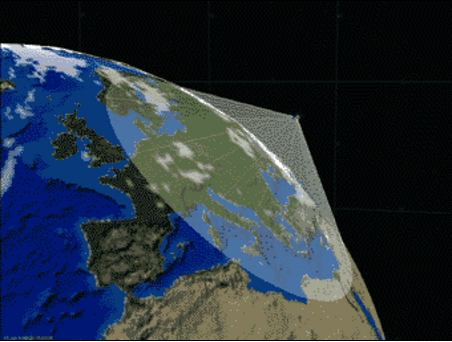
\includegraphics[width=8cm]{noaa}
\centering
\caption[Elevation angle cone]{Elevation angle cone. Source: NOAA}
\end{figure}

\subsection{Elevation angle cone}
Global coverage will be discussed considering the elevation angle and its resulting footprint on Earth. The elevation angle is described by the angular orientation of the antennas in the ground station. However, this angle is also perceived by the satellite in a similar way - it will vary depending on the orientation of the satellite and the angle between horizontal local planes. In order to describe the footprints we must define a cone which vertex is set at the antennas of the satellite, pointing down to Earth, and which generatrix is given by the angle of elevation. This elevation angle based cone is the description of the paths that our communications can take place. In other words, the generatrix of this cone is setting the limits in which the antenna will operate as function of the elevation angle. This implies that our satellite will be able to communicate to all the points contained in the cone. Finally, this cone will be describing a circular surface on top of the Earth which we will call the footprint of the satellite. Additionally, this footprint is the coverage that a single satellite can generate, hence we will be distributing satellites all around the Earth in order to fulfill global coverage. 

\subsection{Atmospheric restrictive conditions}
In order to obtain the final restrictive angle of elevation needed to contact the ground stations some considerations have to be made. First, a description of the different atmospheric conditions will be defined. Then, we will relate these to our bandwidth in order to analyse if they must be taken into account when communicating with ground stations. [elec2013cantero]

\begin{itemize}
\item \textbf{Atmospheric gases: }water vapour and oxygen absorptions; important when frequencies are above 3 GHz. More information [64] and [07328546]
\item \textbf{Precipitations and Clouds: }these conditions are relevant for signals above 10GHz.
\item \textbf{Cross Polarization Discrimination: }direct consequence of both terrestrial links and rain. Related to non-spherical rain drops which have a polarization rotated towards the component of the major axis, and hence may attenuate a signal wave.
\item \textbf{Scintillation } is a rapid fluctuation in signal amplitude at low elevations.
\textendash\textbf{Radio Refracting Index: } for elevation angles below 3 degrees (especially those below 1 degree) and depending on the latitude of our satellite we may find big signal losses due to the resulting differential ray bending.
\end{itemize}

\subsubsubsection*{ Ionosphere layers: }

\textbf{D layers:} 60-90km. Considerable signal absorptions for 10 MHz and below, with progressively less absorption at hihger frequencies and oblique incidencies.

\textbf{E layers:} 90-150 km. Absorptions relevant for frequencies lower than 10 MHz, although for sporadic E propagations this value may be increased to 50MHz.

\textbf{Sporadic E layers:} Reflections of radio waves in this thin-cloud small layer may reach to frequencies up to 225MHz. These layers are usually formed following the E layers altitudes.

\textbf{F layers:} 150-500 km and higher. No absorptions or reflections for these layers. The F2 region allows the longest communication paths, above 210km of altitude.

By means of these physical phenomena we can substract the elevation angle as function of the latitude. However, we must take into account that these physical conditions give a value for the elevation angle which may not be the most restrictive. Global coverage conditions, bandwidths, inclination and the final distribution of our constellation will be considering this elevation angle and viceversa, iteratively.

The ASTREA CONSTELLATION was designed and optimized in order to fulfill global coverage for a constant elevation angle - respect to the latitude - of 20 degrees.

Our constellation will be operating at S-band for telemetry and X-band for data relay. Therefore, the satellites need to be operating up to 10 GHz. This directly implies that physical conditions such as atmospheric gases, precipitations and clouds must be studied when determining the elevation angle needed.

The minimum elevation angle is applied in low latitude regions for constellations based on polar orbits whereas this value is also applied out of the low-latitude region for inclined orbit constellations [a general evaluation criterion]. The minimum elevation angle is a specific value which is equivalent to the maximum elevation angle needed to fulfill coverage at a given latitude, considering that the distance between planes is maximum at the equator and that it is reduced for higher latitude positions.

This elevation angle is maximum in a Walker Delta constellation when the latitude is equal to the orbital inclination angle[a general evaluation criterion]. This means that the limiting restrictive elevation angle that we need in order to fulfill global coverage is defined at latitude equal to 72 degrees, which is the inclination of our constellation. Otherwise, we can define a constant elevation angle that will apply to the equator, which will then be, for this model, the restrictive condition.

Accordingly, the approach considered is that of a constant elevation angle to fulfill global coverage at 20 degrees. This implies that our constellation is configured and distributed in order to optimize coverage both at the equator and at the maximum elevation angle latitude. This value has been contrasted and discussed considering the atmospheric conditions and analysing experimental data, which contemplates also the rotation of the Earth among others.

This constant elevation angle model will be very useful in order to analyse and calcute the distribution of the constellation. Nevertheless, we need to describe in an accurate way the minimum elevation angle respect to the latitude. This is why a different model must be approached.

Thus, we need to describe the elevation angle respect to the latitude of our constellation taking into account all considerations above. First, for a latitude of 0 degrees the value of the minimum elevation angle will be of 10 degrees. In our model we have considered that this value was of constant 20 degrees, so in fact we have redundant global coverage. At latitudes between the equator and 45 degrees our second model increases linearly to 15 degrees. From 45 to 60 degrees the elevation angle also increases linearly to 22 degrees. Then, from 60 to 70 tha value increases highly reaching a peak at 70 degrees, where the elevation angle will be of 30 degrees. Finally, from 70 to 80 degrees this model is reduced linearly to 15 degrees, and from 80 to the north and south poles it falls to 0 degrees. This is a simple model that will guarantee global coverage, especially at the latitudes of our ground stations

For the distribution of ground stations we need to guarantee that these will be covered either by one satellite or two at any given moment. As discussed before, the model used was based on a constant 20 degree constant elevation angle. However, for this last model that we have described - which is more realistic - we obtain more coverage than for the constant model except for those regions next to the peak. The most restrictive latitude is now 60 degrees - where all the ground stations are set - and has a 22 degree restriction of the angle of elevation, which is higher than the constant model described previously. These facts imply the following:

\begin{itemize}
\item At low latitudes (between 0 and 30 degrees) the constellation fulfills global coverage generously.
\item At ground station latitude (60 degrees) the constellation is covering the station succesfully. As discussed before, our first model considered a constant 20 degree elevation angle instead of the 22 degrees that now must be corrected. For the previous model coverage was well established with margin. For the latter, the margin has decreased but coverage is still complete. Note: each orbit could be reduced by a number of satellites per plane, but this would endanger the correct and stationary working of the constellation. In this case we would not be able to control possible incidencies such as unoperative satellites with enough margin.
\item The ground stations are covered at all time for at least one satellite.
\end{itemize}

\subsection{Elevation angle of other current constellations}

Analysing the minimum elevation angle needed in order to fulfill global coverage requieres, as mentioned before, the understanding first of the restrictive conditions of the atmosphere and how these will alter it. As a consequence of the different physical conditions given before we will be able to determine a relation between latitude and elevation angle. All the same, the elevation angle depends on the bandwith in which the satellites operate, hence different distributions of this angle respect to the latitude will be described depending on the bandwidths used. 

\begin{itemize}
\item Celestri: 18.8 to 20.2 GHz at 48 degree inclination.
\item GlobalStar: 2.4 GHz at 52 degree inclination.
\item Iridium: 20 to 30 GHz at 90 degree inclination - polar orbits.
\end{itemie}

Comparing our configuration to other present constellations some clarifications can be made: 

\begin{itemize}
\item The minimum elevation angle peak is proportional to the bandwidth at which the satellite is communicating with Earth. For instance, Iridium's peak of elevation angle is the highest relative to the other configurations since it is also working with the highest frequency signals.
\item The latitude position of the peaks is related to the inclination of the constellation. Iridium, - a polar orbit based configuration - describes a peak at 90 degrees of latitude whereas Celestri and GlobalStar are near 40 to 50 degrees.
\end{itemize}

With these tendencies our model can be confirmed as function of the frequencies of the signals and related to the inclination of the orbits. 

\begin{figure}[H]
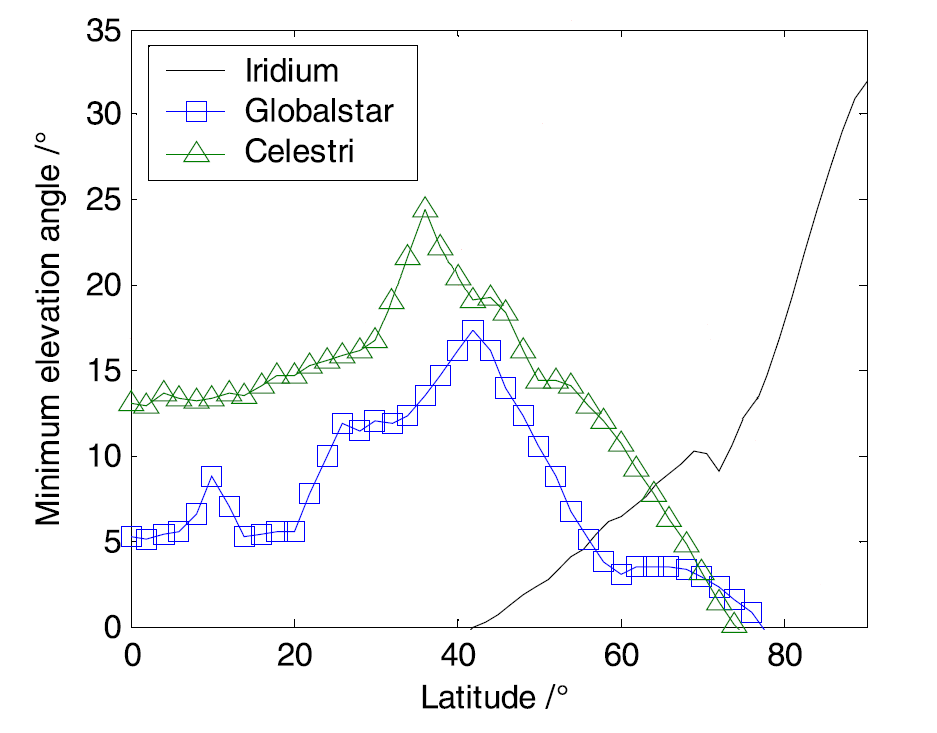
\includegraphics[width=8cm]{latitudes}
\centering
\caption[Minimum elevation angle as function of latitude]{Minimum elevation angle as function of latitude. Source: [a general evaluation criterion]}
\end{figure}